Chương này trình bày quá trình hiện thực hóa hệ thống chatbot hỗ trợ tra
cứu TTHC cho tỉnh Lai Châu sau giai đoạn phân tích và thiết kế. Nội dung
chương được tổ chức theo trình tự triển khai thực tế: cài đặt backend,
cài đặt frontend, bảo vệ hệ thống, quản trị kho tri thức, kiểm thử chức
năng, đánh giá chatbot RAG và hướng dẫn sử dụng.

Trọng tâm của chương không chỉ là mô tả cách chạy hệ thống mà còn thể
hiện minh chứng vận hành và kết quả đánh giá trên bộ 100 câu hỏi thử
nghiệm. Các kết quả đánh giá được ghi nhận từ file chạy test API, gồm
câu hỏi, câu trả lời thực tế, thời gian phản hồi và nhận xét đối chiếu
với dữ liệu nguồn.

\section{Cài đặt backend và pipeline
RAG}

Backend là thành phần trung tâm của hệ thống. Mọi luồng quan trọng đều
đi qua backend: nhận câu hỏi, kiểm tra đăng nhập, lấy lịch sử hội thoại,
chạy pipeline RAG, gọi mô hình ngôn ngữ, lưu kết quả và xử lý chức năng
quản trị. Quá trình cài đặt backend gồm tạo môi trường ảo Python, cài
thư viện từ requirements.txt, cấu hình .env, đặt serviceAccountKey.json
ở phía backend và chuẩn bị thư mục data chứa procedures.json,
entities.json, synonyms.json, intents.json và all\_laichau\_codes.json.

\section{Cài đặt frontend và kết nối
API}

Frontend là phần người dùng trực tiếp thao tác. Giao diện được tổ chức
theo các component chính như LoginPage, ChatBox, Sidebar, InputBox,
Message và AdminDashboard. Cách chia component giúp quá trình phát
triển, kiểm thử và mở rộng giao diện thuận lợi hơn.

\begin{longtable}[]{|
  >{\raggedright\arraybackslash}p{(\columnwidth - 4\tabcolsep) * \real{0.1651}}|
  >{\raggedright\arraybackslash}p{(\columnwidth - 4\tabcolsep) * \real{0.2568}}|
  >{\raggedright\arraybackslash}p{(\columnwidth - 4\tabcolsep) * \real{0.5781}}|}
\caption{API chính frontend sử dụng}\\
\hline
\begin{minipage}[b]{\linewidth}\raggedright
\textbf{Nhóm}
\end{minipage} & \begin{minipage}[b]{\linewidth}\raggedright
\textbf{Endpoint}
\end{minipage} & \begin{minipage}[b]{\linewidth}\raggedright
\textbf{Mục đích}
\end{minipage} \\
\hline
\endfirsthead
\continuedcaption{API chính frontend sử dụng}
\hline
\begin{minipage}[b]{\linewidth}\raggedright
\textbf{Nhóm}
\end{minipage} & \begin{minipage}[b]{\linewidth}\raggedright
\textbf{Endpoint}
\end{minipage} & \begin{minipage}[b]{\linewidth}\raggedright
\textbf{Mục đích}
\end{minipage} \\
\hline
\endhead
\hline
\endlastfoot
Auth & /auth/send-otp & Gửi mã OTP khi người dùng đăng ký bằng email. \\
\hline
Auth & /auth/verify-otp & Xác minh OTP và hoàn tất tạo tài khoản. \\
\hline
Auth & /auth/check-admin & Kiểm tra tài khoản hiện tại có quyền admin
hay không. \\
\hline
User & /user/chat & Gửi câu hỏi đến chatbot và nhận câu trả lời. \\
\hline
User & /user/sessions & Lấy danh sách phiên hội thoại. \\
\hline
User & /user/chat/history & Lấy lại tin nhắn trong một phiên chat. \\
\hline
Admin & /admin/stats & Lấy số liệu thống kê và dữ liệu biểu đồ. \\
\hline
Admin & /admin/documents & Quản lý dữ liệu thủ tục hành chính. \\
\hline
Admin & /admin/convert-json & Dùng AI trích xuất văn bản thô thành
JSON. \\
\hline
Admin & /admin/reload-vectordb & Đồng bộ lại ChromaDB sau khi dữ liệu
thay đổi. \\
\hline
Admin & /admin/backups & Liệt kê hoặc xóa bản sao lưu VectorDB. \\
\hline
\end{longtable}

\emph{Backend được khởi chạy bằng Uvicorn, frontend được chạy bằng Vite
và backend có thể mở ra môi trường thử nghiệm bằng ngrok (xem các lệnh
chạy hệ thống tại Phụ lục B).}

\section{Bảo vệ hệ thống và dữ
liệu}

Hệ thống lưu lịch sử hội thoại và có khu vực quản trị, vì vậy cơ chế bảo
vệ phải được đặt ở backend. Mọi request cần bảo vệ đều sử dụng Firebase
ID Token và được backend xác minh trước khi xử lý. Các chức năng quản
trị tiếp tục kiểm tra email admin để tránh người dùng thường gọi trực
tiếp API quản trị.

\begin{figure}[H]
\centering
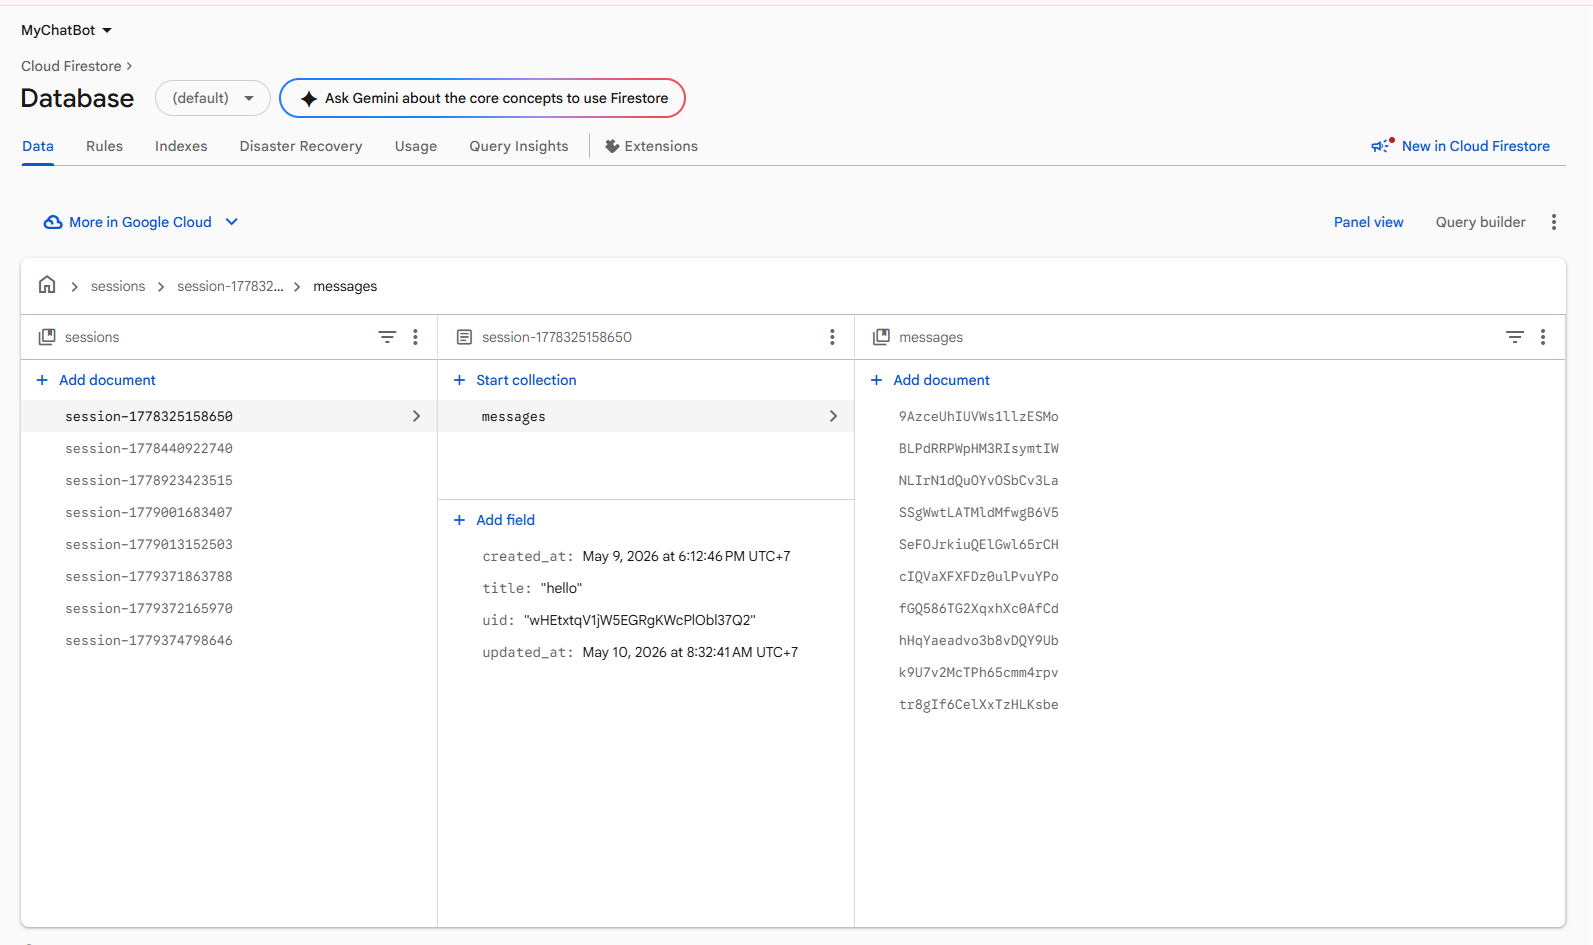
\includegraphics[width=0.92\textwidth]{tai_nguyen/media/image25.png}
\caption{Minh chứng Firestore lưu phiên hội thoại và tin nhắn}
\label{fig:4-1}
\end{figure}

\begin{longtable}[]{|
  >{\raggedright\arraybackslash}p{(\columnwidth - 4\tabcolsep) * \real{0.1823}}|
  >{\raggedright\arraybackslash}p{(\columnwidth - 4\tabcolsep) * \real{0.4415}}|
  >{\raggedright\arraybackslash}p{(\columnwidth - 4\tabcolsep) * \real{0.3762}}|}
\caption{Checklist bảo vệ khi triển khai}\\
\hline
\begin{minipage}[b]{\linewidth}\raggedright
\textbf{Hạng mục}
\end{minipage} & \begin{minipage}[b]{\linewidth}\raggedright
\textbf{Cách triển khai}
\end{minipage} & \begin{minipage}[b]{\linewidth}\raggedright
\textbf{Mục đích}
\end{minipage} \\
\hline
\endfirsthead
\continuedcaption{Checklist bảo vệ khi triển khai}
\hline
\begin{minipage}[b]{\linewidth}\raggedright
\textbf{Hạng mục}
\end{minipage} & \begin{minipage}[b]{\linewidth}\raggedright
\textbf{Cách triển khai}
\end{minipage} & \begin{minipage}[b]{\linewidth}\raggedright
\textbf{Mục đích}
\end{minipage} \\
\hline
\endhead
\hline
\endlastfoot
Token người dùng & Verify Firebase ID Token ở backend & Tránh giả mạo
đăng nhập. \\
\hline
Quyền admin & Kiểm tra email admin trước khi chạy API quản trị & Ngăn
người dùng thường sửa dữ liệu hoặc reload VectorDB. \\
\hline
OTP đăng ký & Lưu OTP có thời hạn và xác minh trước khi tạo tài khoản &
Giảm tài khoản ảo và kiểm tra quyền sở hữu email. \\
\hline
Khóa dịch vụ & Đặt API key và service account ở backend/secret & Tránh
lộ khóa khi nộp mã nguồn hoặc deploy frontend. \\
\hline
Dữ liệu hội thoại & Lưu theo uid/session\_id và giới hạn lịch sử đưa vào
prompt & Giảm rủi ro lộ dữ liệu cá nhân. \\
\hline
VectorDB & Backup trước khi reload và dọn backup quá hạn & Có điểm khôi
phục khi build dữ liệu lỗi. \\
\hline
\end{longtable}

\section{Hoạt động thử nghiệm, kiểm thử và
đánh giá định
lượng}

Kiểm thử hệ thống RAG cần bao phủ cả phần mềm truyền thống và chất lượng
AI. Với phần mềm truyền thống, các luồng xác thực, lưu lịch sử, phân
quyền admin, quản lý dữ liệu và reload VectorDB được kiểm thử bằng kịch
bản đầu vào - kết quả mong đợi. Với chatbot RAG, quá trình đánh giá sử
dụng bộ 100 câu hỏi để xem xét độ đúng của câu trả lời, khả năng từ chối
ngoài phạm vi và thời gian phản hồi.

\begin{longtable}[]{|
  >{\raggedright\arraybackslash}p{(\columnwidth - 10\tabcolsep) * \real{0.1467}}|
  >{\raggedright\arraybackslash}p{(\columnwidth - 10\tabcolsep) * \real{0.1282}}|
  >{\raggedright\arraybackslash}p{(\columnwidth - 10\tabcolsep) * \real{0.1995}}|
  >{\raggedright\arraybackslash}p{(\columnwidth - 10\tabcolsep) * \real{0.2105}}|
  >{\raggedright\arraybackslash}p{(\columnwidth - 10\tabcolsep) * \real{0.2146}}|
  >{\raggedright\arraybackslash}p{(\columnwidth - 10\tabcolsep) * \real{0.1004}}|}
\caption{Kịch bản kiểm thử chức năng có minh chứng}\\
\hline
\begin{minipage}[b]{\linewidth}\raggedright
\textbf{Mã ca}
\end{minipage} & \begin{minipage}[b]{\linewidth}\raggedright
\textbf{Kịch bản}
\end{minipage} & \begin{minipage}[b]{\linewidth}\raggedright
\textbf{Dữ liệu đầu vào}
\end{minipage} & \begin{minipage}[b]{\linewidth}\raggedright
\textbf{Kết quả mong đợi}
\end{minipage} & \begin{minipage}[b]{\linewidth}\raggedright
\textbf{Minh chứng}
\end{minipage} & \begin{minipage}[b]{\linewidth}\raggedright
\textbf{Trạng thái}
\end{minipage} \\
\hline
\endfirsthead
\continuedcaption{Kịch bản kiểm thử chức năng có minh chứng}
\hline
\begin{minipage}[b]{\linewidth}\raggedright
\textbf{Mã ca}
\end{minipage} & \begin{minipage}[b]{\linewidth}\raggedright
\textbf{Kịch bản}
\end{minipage} & \begin{minipage}[b]{\linewidth}\raggedright
\textbf{Dữ liệu đầu vào}
\end{minipage} & \begin{minipage}[b]{\linewidth}\raggedright
\textbf{Kết quả mong đợi}
\end{minipage} & \begin{minipage}[b]{\linewidth}\raggedright
\textbf{Minh chứng}
\end{minipage} & \begin{minipage}[b]{\linewidth}\raggedright
\textbf{Trạng thái}
\end{minipage} \\
\hline
\endhead
\hline
\endlastfoot
AUTH\_01 & Đăng ký email mới và sinh OTP & Email hợp lệ, mật khẩu hợp lệ
& Sinh OTP, lưu tạm trong Firestore và cho phép xác minh tài khoản. &
Ảnh Firebase Auth/Firestore, màn hình OTP & Đạt \\
\hline
AUTH\_02 & Truy cập API không có token & Không gửi Authorization header
& Backend từ chối request bằng lỗi xác thực. & Response API hoặc
Swagger/log backend & Đạt \\
\hline
CHAT\_01 & Hỏi hồ sơ thủ tục cụ thể & Giải quyết chế độ mai táng phí đối
với cựu chiến binh cần giấy tờ gì? & Chatbot trả lời theo thành phần hồ
sơ từ dữ liệu nguồn. & Ảnh màn hình chatbot và dòng kết quả trong CSV &
Đạt \\
\hline
CHAT\_02 & Câu hỏi tiếp nối & Ngữ cảnh trước + câu hỏi: Thế lệ phí bao
nhiêu? & Chatbot dùng lịch sử để hiểu thủ tục đang hỏi. & Kết quả TC 081
trong file test & Đạt \\
\hline
CHAT\_03 & Câu hỏi ngoài phạm vi & Dự đoán giá vàng hoặc kết quả xổ số &
Chatbot từ chối, không tự bịa thủ tục. & Kết quả TC 096-TC\_100 & Đạt \\
\hline
ADM\_01 & Xem thống kê hệ thống & Tài khoản admin hợp lệ & Dashboard
hiển thị số liệu và biểu đồ. & Ảnh trang thống kê admin & Đạt \\
\hline
ADM\_02 & Quản lý dữ liệu thủ tục & JSON thủ tục hợp lệ & Dữ liệu được
cập nhật và có thể reload VectorDB. & Ảnh quản lý dữ liệu và reload
VectorDB & Đạt \\
\hline
\end{longtable}

\begin{longtable}[]{|
  >{\raggedright\arraybackslash}p{(\columnwidth - 2\tabcolsep) * \real{0.5007}}|
  >{\raggedright\arraybackslash}p{(\columnwidth - 2\tabcolsep) * \real{0.4993}}|}
\caption{Phân nhóm bộ 100 câu hỏi thử nghiệm chatbot RAG}\\
\hline
\begin{minipage}[b]{\linewidth}\raggedright
\textbf{Nhóm}
\end{minipage} & \begin{minipage}[b]{\linewidth}\raggedright
\textbf{Số lượng}
\end{minipage} \\
\hline
\endfirsthead
\continuedcaption{Phân nhóm bộ 100 câu hỏi thử nghiệm chatbot RAG}
\hline
\begin{minipage}[b]{\linewidth}\raggedright
\textbf{Nhóm}
\end{minipage} & \begin{minipage}[b]{\linewidth}\raggedright
\textbf{Số lượng}
\end{minipage} \\
\hline
\endhead
\hline
\endlastfoot
Thành phần hồ sơ & 15 \\
\hline
Thời hạn giải quyết & 15 \\
\hline
Phí/lệ phí & 15 \\
\hline
Cơ quan thực hiện & 10 \\
\hline
Cách thức thực hiện & 10 \\
\hline
Căn cứ pháp lý & 10 \\
\hline
Kết quả thực hiện & 5 \\
\hline
Hội thoại tiếp nối & 5 \\
\hline
Câu hỏi bẫy/gây nhiễu & 10 \\
\hline
Ngoài phạm vi & 5 \\
\hline
\end{longtable}

\emph{Bảng 4.4 cho biết cách phân bố 100 câu hỏi theo từng nhóm nội dung
đánh giá. Danh sách đầy đủ 100 câu hỏi kiểm thử, kết quả đánh giá, thời
gian phản hồi và điểm hiệu năng của từng test được trình bày tại Phụ lục
D.}

\begin{figure}[H]
\centering
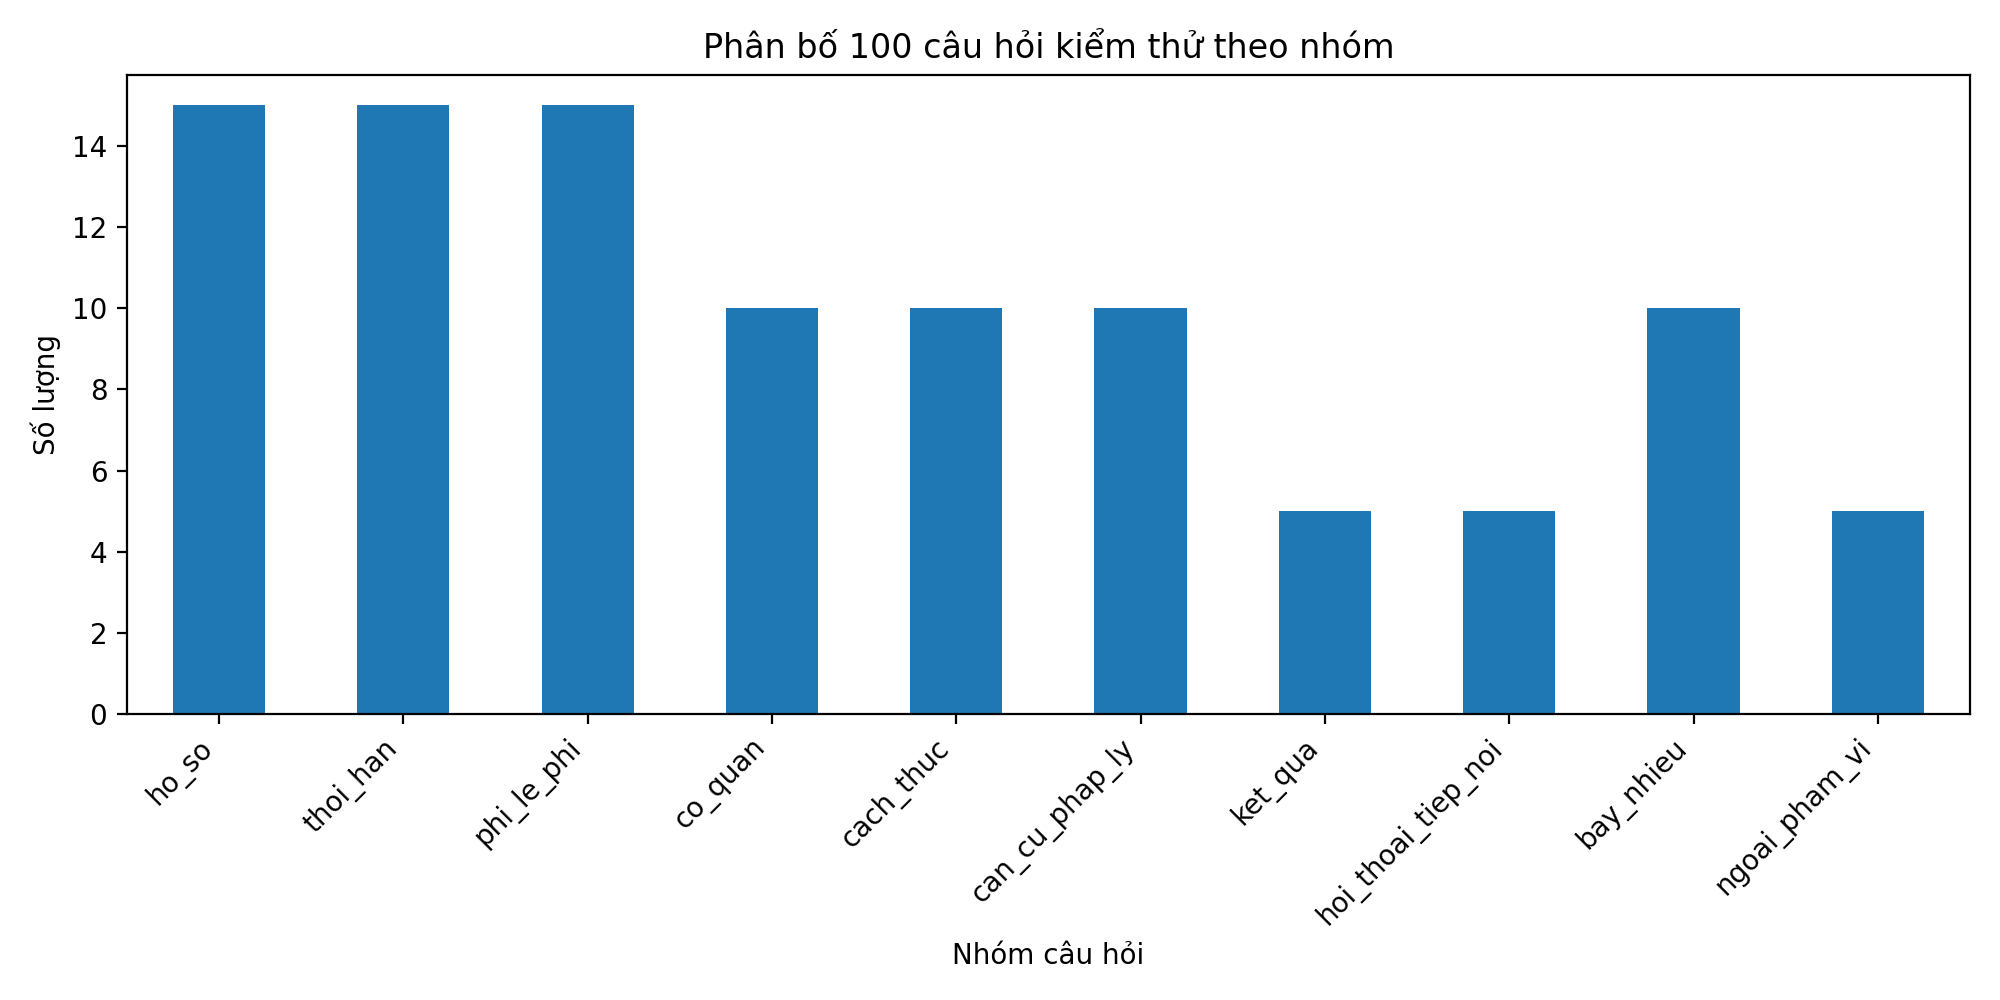
\includegraphics[width=0.92\textwidth]{tai_nguyen/media/image26.png}
\caption{Biểu đồ phân bố 100 câu hỏi kiểm thử theo nhóm}
\label{fig:4-2}
\end{figure}

\begin{longtable}[]{|
  >{\raggedright\arraybackslash}p{(\columnwidth - 4\tabcolsep) * \real{0.2561}}|
  >{\raggedright\arraybackslash}p{(\columnwidth - 4\tabcolsep) * \real{0.1852}}|
  >{\raggedright\arraybackslash}p{(\columnwidth - 4\tabcolsep) * \real{0.5587}}|}
\caption{Kết quả đánh giá định lượng chatbot RAG}\\
\hline
\begin{minipage}[b]{\linewidth}\raggedright
\textbf{Chỉ số}
\end{minipage} & \begin{minipage}[b]{\linewidth}\raggedright
\textbf{Kết quả ghi nhận}
\end{minipage} & \begin{minipage}[b]{\linewidth}\raggedright
\textbf{Nhận xét}
\end{minipage} \\
\hline
\endfirsthead
\continuedcaption{Kết quả đánh giá định lượng chatbot RAG}
\hline
\begin{minipage}[b]{\linewidth}\raggedright
\textbf{Chỉ số}
\end{minipage} & \begin{minipage}[b]{\linewidth}\raggedright
\textbf{Kết quả ghi nhận}
\end{minipage} & \begin{minipage}[b]{\linewidth}\raggedright
\textbf{Nhận xét}
\end{minipage} \\
\hline
\endhead
\hline
\endlastfoot
Số câu hỏi kiểm thử & 100 câu & Bộ test được sinh từ dữ liệu
procedures.json. \\
\hline
Câu trả lời đúng & 82/100 (82.0\%) & Chỉ tính các câu trả lời đúng hoặc
từ chối đúng. \\
\hline
Câu trả lời chấp nhận được & 92/100 (92.0\%) & Gồm đúng, đúng nhưng
thiếu ý và từ chối đúng. \\
\hline
Từ chối đúng ngoài phạm vi & 5/5 (100.0\%) & Áp dụng cho nhóm câu hỏi
ngoài phạm vi. \\
\hline
Latency trung bình & 16.49 giây & Đo từ lúc gửi request đến khi nhận
response. \\
\hline
Latency nhỏ nhất & 6.63 giây & Ghi nhận trong file kết quả test. \\
\hline
Latency lớn nhất & 51.33 giây & Truy vấn chậm nhất trong bộ 100 câu. \\
\hline
Latency P95 & 34.79 giây & 95\% số câu có thời gian phản hồi không vượt
quá giá trị này. \\
\hline
Top-k retrieval accuracy & Chưa đo trực tiếp & API hiện chưa trả danh
sách chunk/sources hoặc log top-k nên chưa tính chính xác từ file kết
quả hiện có. \\
\hline
\end{longtable}

\begin{figure}[H]
\centering
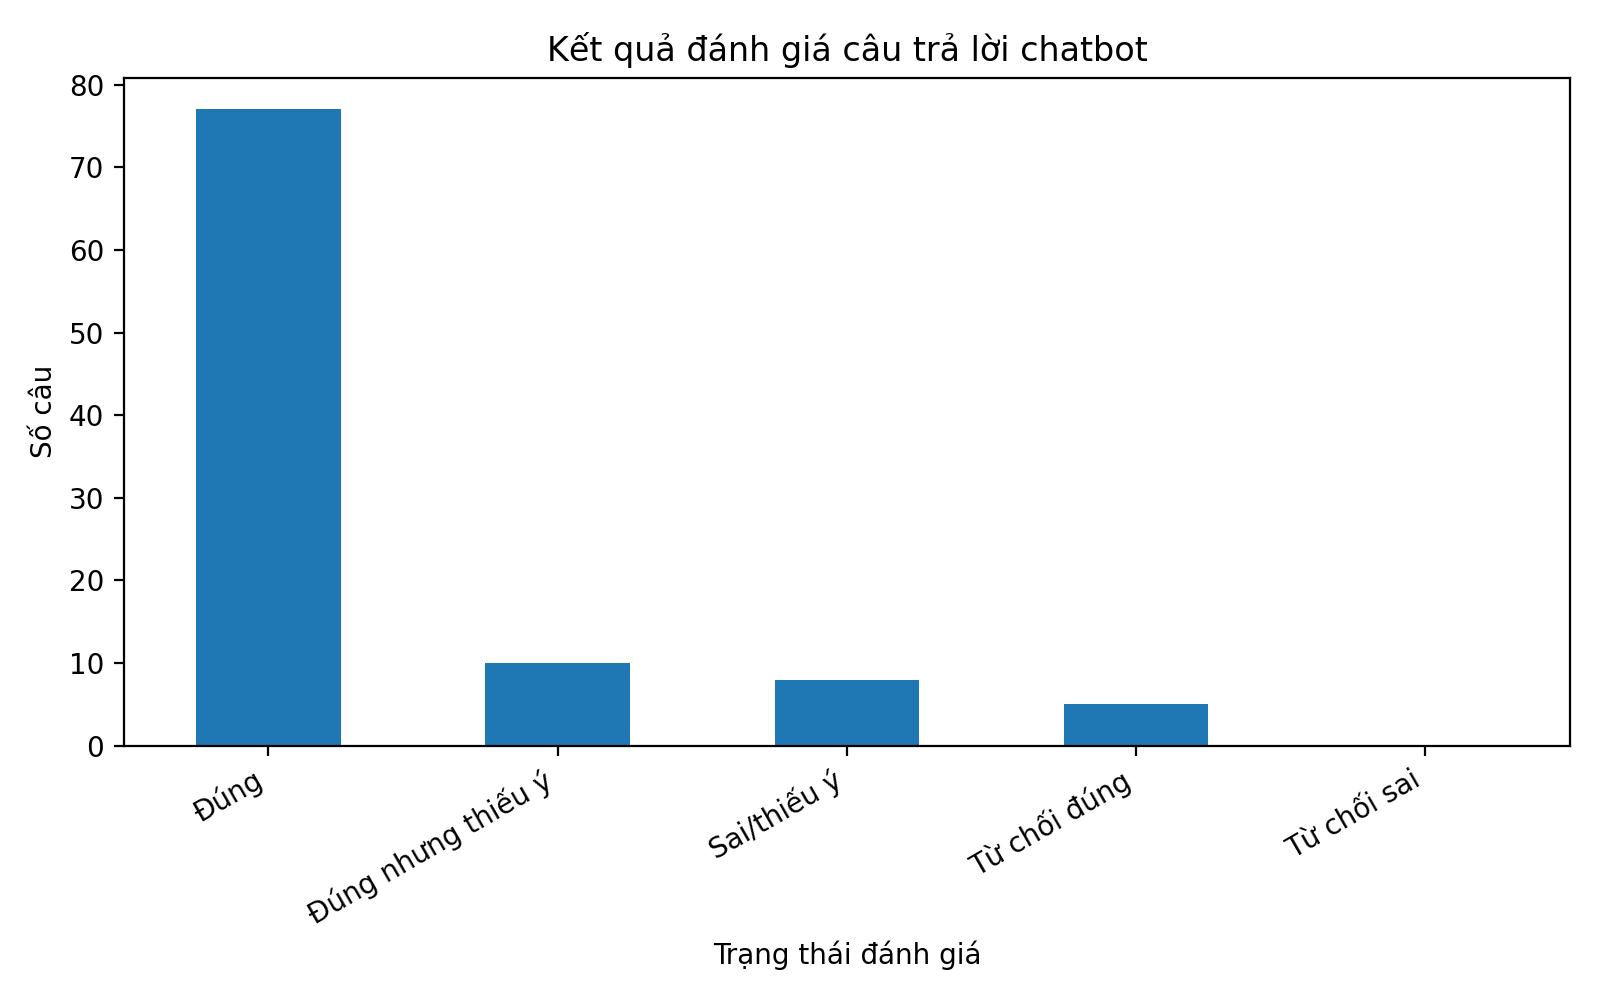
\includegraphics[width=0.92\textwidth]{tai_nguyen/media/image27.png}
\caption{Kết quả đánh giá câu trả lời chatbot}
\label{fig:4-3}
\end{figure}

\begin{figure}[H]
\centering
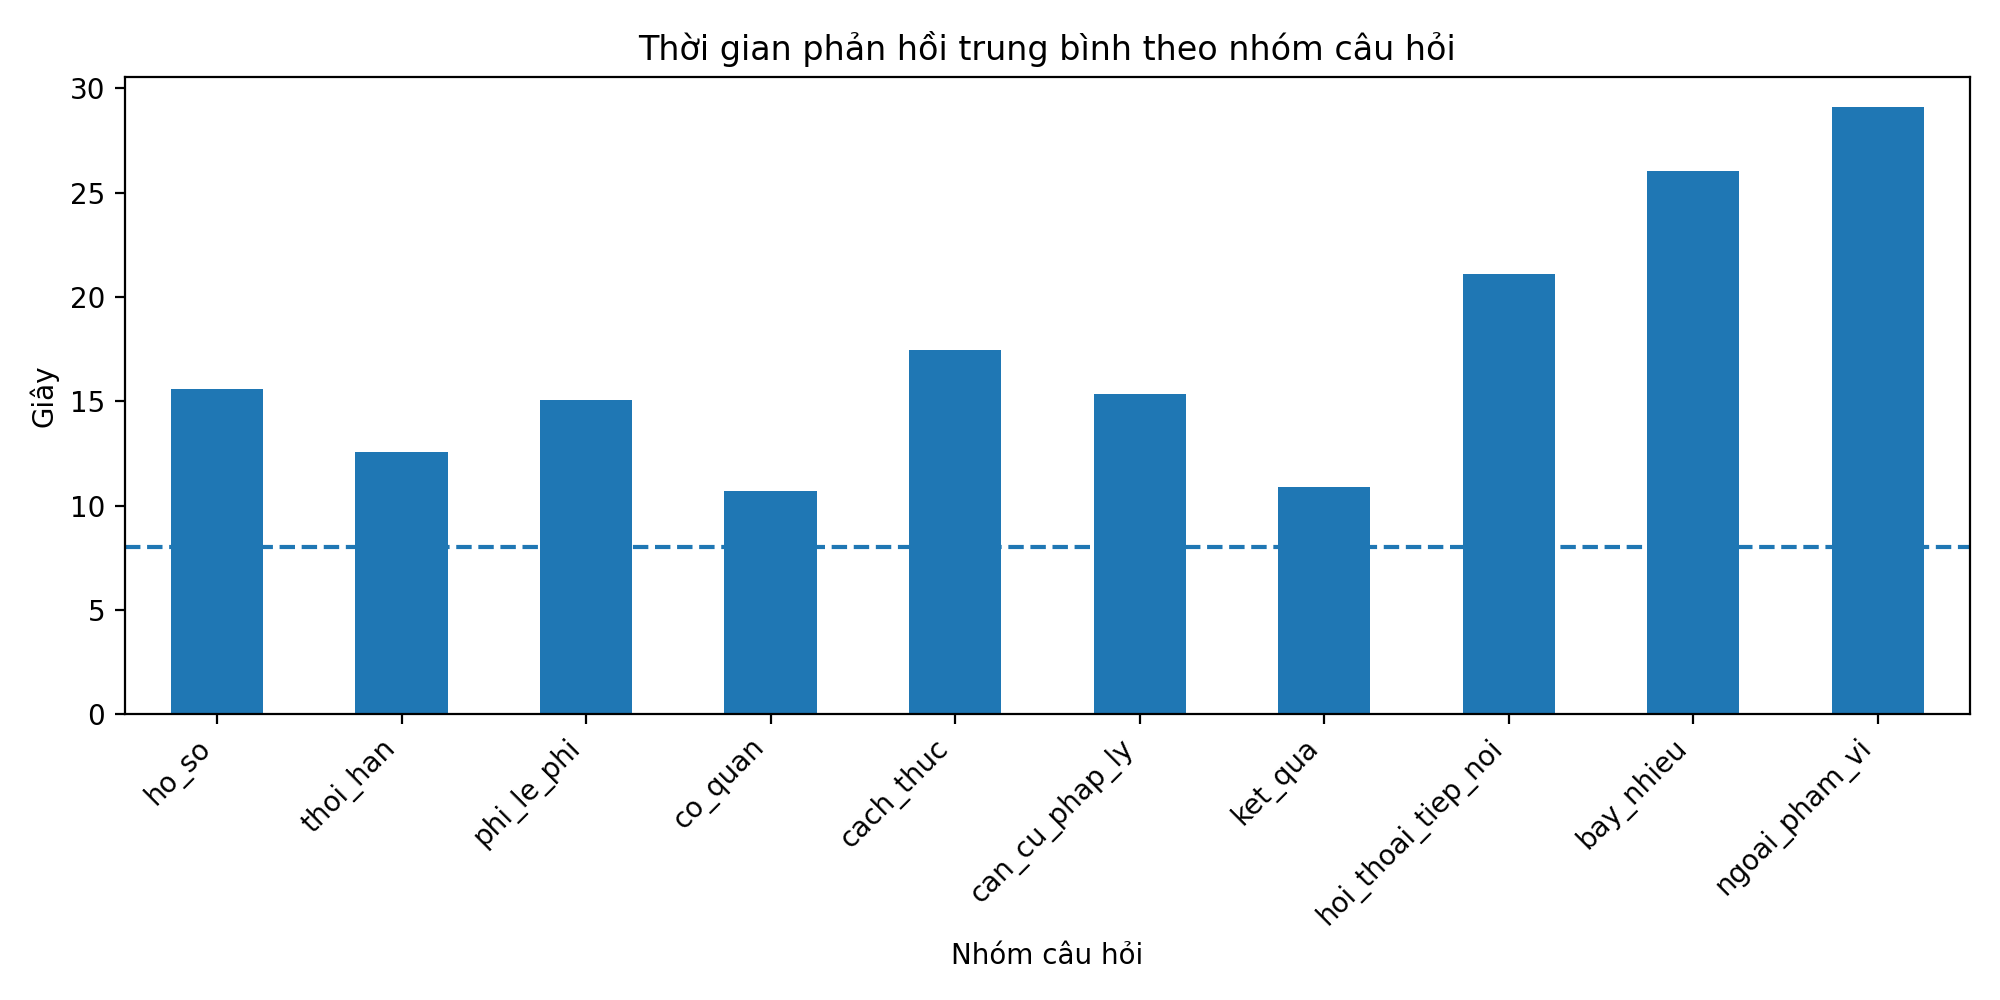
\includegraphics[width=0.92\textwidth]{tai_nguyen/media/image28.png}
\caption{Thời gian phản hồi trung bình theo nhóm câu hỏi}
\label{fig:4-4}
\end{figure}

\begin{longtable}[]{|
  >{\raggedright\arraybackslash}p{(\columnwidth - 10\tabcolsep) * \real{0.2242}}|
  >{\raggedright\arraybackslash}p{(\columnwidth - 10\tabcolsep) * \real{0.0936}}|
  >{\raggedright\arraybackslash}p{(\columnwidth - 10\tabcolsep) * \real{0.2122}}|
  >{\raggedright\arraybackslash}p{(\columnwidth - 10\tabcolsep) * \real{0.1403}}|
  >{\raggedright\arraybackslash}p{(\columnwidth - 10\tabcolsep) * \real{0.1670}}|
  >{\raggedright\arraybackslash}p{(\columnwidth - 10\tabcolsep) * \real{0.1628}}|}
\caption{Tổng hợp trạng thái đánh giá theo nhóm câu hỏi}\\
\hline
\begin{minipage}[b]{\linewidth}\raggedright
\textbf{Nhóm}
\end{minipage} & \begin{minipage}[b]{\linewidth}\raggedright
\textbf{Đúng}
\end{minipage} & \begin{minipage}[b]{\linewidth}\raggedright
\textbf{Đúng nhưng thiếu ý}
\end{minipage} & \begin{minipage}[b]{\linewidth}\raggedright
\textbf{Sai/thiếu ý}
\end{minipage} & \begin{minipage}[b]{\linewidth}\raggedright
\textbf{Từ chối đúng}
\end{minipage} & \begin{minipage}[b]{\linewidth}\raggedright
\textbf{Từ chối sai}
\end{minipage} \\
\hline
\endfirsthead
\continuedcaption{Tổng hợp trạng thái đánh giá theo nhóm câu hỏi}
\hline
\begin{minipage}[b]{\linewidth}\raggedright
\textbf{Nhóm}
\end{minipage} & \begin{minipage}[b]{\linewidth}\raggedright
\textbf{Đúng}
\end{minipage} & \begin{minipage}[b]{\linewidth}\raggedright
\textbf{Đúng nhưng thiếu ý}
\end{minipage} & \begin{minipage}[b]{\linewidth}\raggedright
\textbf{Sai/thiếu ý}
\end{minipage} & \begin{minipage}[b]{\linewidth}\raggedright
\textbf{Từ chối đúng}
\end{minipage} & \begin{minipage}[b]{\linewidth}\raggedright
\textbf{Từ chối sai}
\end{minipage} \\
\hline
\endhead
\hline
\endlastfoot
Câu hỏi bẫy/gây nhiễu & 5 & 1 & 4 & 0 & 0 \\
\hline
Cách thức thực hiện & 10 & 0 & 0 & 0 & 0 \\
\hline
Căn cứ pháp lý & 8 & 1 & 1 & 0 & 0 \\
\hline
Cơ quan thực hiện & 9 & 0 & 1 & 0 & 0 \\
\hline
Thành phần hồ sơ & 10 & 4 & 1 & 0 & 0 \\
\hline
Hội thoại tiếp nối & 4 & 1 & 0 & 0 & 0 \\
\hline
Kết quả thực hiện & 5 & 0 & 0 & 0 & 0 \\
\hline
Ngoài phạm vi & 0 & 0 & 0 & 5 & 0 \\
\hline
Phí/lệ phí & 15 & 0 & 0 & 0 & 0 \\
\hline
Thời hạn giải quyết & 11 & 3 & 1 & 0 & 0 \\
\hline
\end{longtable}

\begin{longtable}[]{|
  >{\raggedright\arraybackslash}p{(\columnwidth - 4\tabcolsep) * \real{0.3478}}|
  >{\raggedright\arraybackslash}p{(\columnwidth - 4\tabcolsep) * \real{0.1366}}|
  >{\raggedright\arraybackslash}p{(\columnwidth - 4\tabcolsep) * \real{0.5156}}|}
\caption{So sánh kết quả với baseline tìm kiếm từ khóa mô phỏng}\\
\hline
\begin{minipage}[b]{\linewidth}\raggedright
\textbf{Phương án/chỉ số}
\end{minipage} & \begin{minipage}[b]{\linewidth}\raggedright
\textbf{Kết quả}
\end{minipage} & \begin{minipage}[b]{\linewidth}\raggedright
\textbf{Ghi chú}
\end{minipage} \\
\hline
\endfirsthead
\continuedcaption{So sánh kết quả với baseline tìm kiếm từ khóa mô phỏng}
\hline
\begin{minipage}[b]{\linewidth}\raggedright
\textbf{Phương án/chỉ số}
\end{minipage} & \begin{minipage}[b]{\linewidth}\raggedright
\textbf{Kết quả}
\end{minipage} & \begin{minipage}[b]{\linewidth}\raggedright
\textbf{Ghi chú}
\end{minipage} \\
\hline
\endhead
\hline
\endlastfoot
Tìm kiếm từ khóa mô phỏng - Top 1 & 24.2\% & Tính bằng trùng khớp từ
khóa trên tên/nội dung thủ tục. \\
\hline
Tìm kiếm từ khóa mô phỏng - Top 3 & 42.1\% & Kiểm tra thủ tục kỳ vọng có
nằm trong 3 kết quả đầu. \\
\hline
Tìm kiếm từ khóa mô phỏng - Top 5 & 53.7\% & Kiểm tra thủ tục kỳ vọng có
nằm trong 5 kết quả đầu. \\
\hline
Chatbot RAG - trả lời đúng & 82.0\% & Đánh giá theo câu trả lời thực tế
của hệ thống. \\
\hline
Chatbot RAG - chấp nhận được & 92.0\% & Tính cả các câu đúng nhưng thiếu
ý. \\
\hline
\end{longtable}

\begin{figure}[H]
\centering
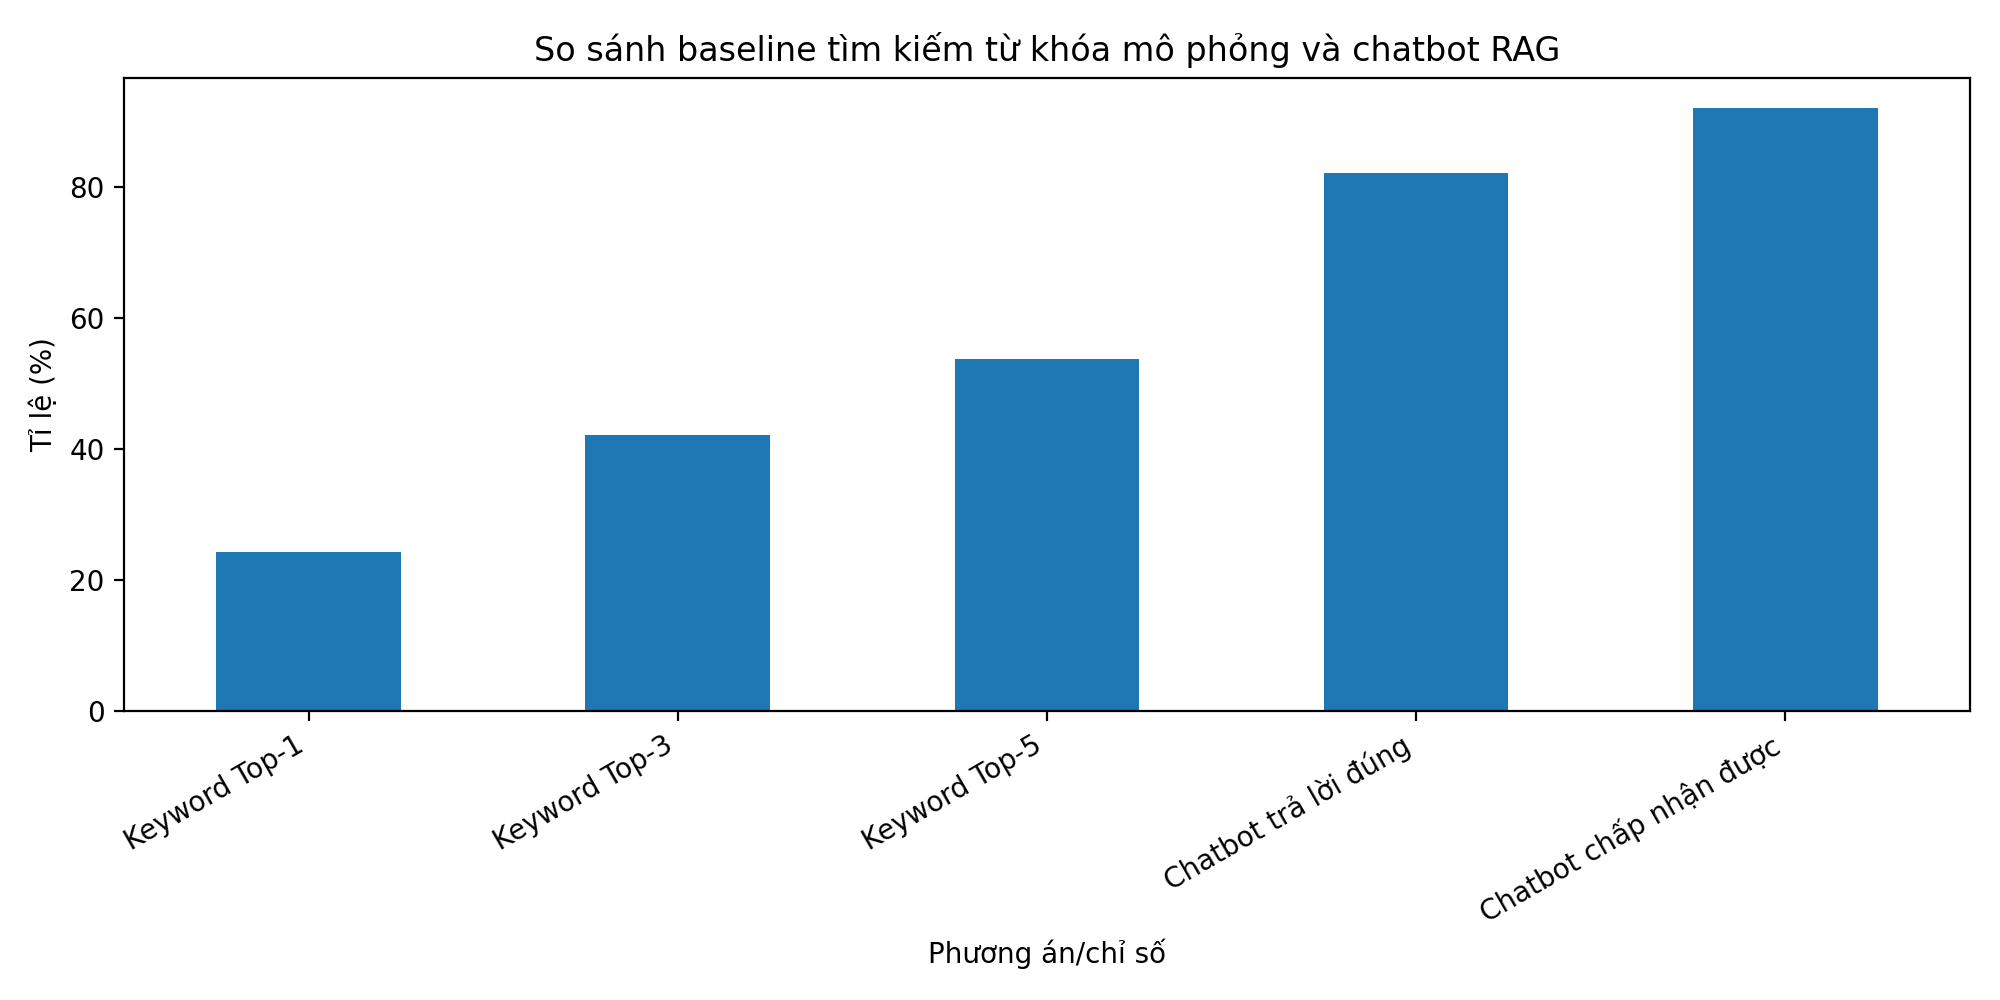
\includegraphics[width=0.92\textwidth]{tai_nguyen/media/image29.png}
\caption{So sánh baseline tìm kiếm từ khóa mô phỏng và chatbot RAG}
\label{fig:4-5}
\end{figure}

\begin{longtable}[]{|
  >{\raggedright\arraybackslash}p{(\columnwidth - 10\tabcolsep) * \real{0.0777}}|
  >{\raggedright\arraybackslash}p{(\columnwidth - 10\tabcolsep) * \real{0.1095}}|
  >{\raggedright\arraybackslash}p{(\columnwidth - 10\tabcolsep) * \real{0.3442}}|
  >{\raggedright\arraybackslash}p{(\columnwidth - 10\tabcolsep) * \real{0.1062}}|
  >{\raggedright\arraybackslash}p{(\columnwidth - 10\tabcolsep) * \real{0.1284}}|
  >{\raggedright\arraybackslash}p{(\columnwidth - 10\tabcolsep) * \real{0.2341}}|}
\caption{Một số kết quả kiểm thử đại diện sau khi chạy API}\\
\hline
\begin{minipage}[b]{\linewidth}\raggedright
\textbf{Mã}
\end{minipage} & \begin{minipage}[b]{\linewidth}\raggedright
\textbf{Nhóm}
\end{minipage} & \begin{minipage}[b]{\linewidth}\raggedright
\textbf{Câu hỏi}
\end{minipage} & \begin{minipage}[b]{\linewidth}\raggedright
\textbf{Đánh giá}
\end{minipage} & \begin{minipage}[b]{\linewidth}\raggedright
\textbf{Latency (ms)}
\end{minipage} & \begin{minipage}[b]{\linewidth}\raggedright
\textbf{Nhận xét}
\end{minipage} \\
\hline
\endfirsthead
\continuedcaption{Một số kết quả kiểm thử đại diện sau khi chạy API}
\hline
\begin{minipage}[b]{\linewidth}\raggedright
\textbf{Mã}
\end{minipage} & \begin{minipage}[b]{\linewidth}\raggedright
\textbf{Nhóm}
\end{minipage} & \begin{minipage}[b]{\linewidth}\raggedright
\textbf{Câu hỏi}
\end{minipage} & \begin{minipage}[b]{\linewidth}\raggedright
\textbf{Đánh giá}
\end{minipage} & \begin{minipage}[b]{\linewidth}\raggedright
\textbf{Latency (ms)}
\end{minipage} & \begin{minipage}[b]{\linewidth}\raggedright
\textbf{Nhận xét}
\end{minipage} \\
\hline
\endhead
\hline
\endlastfoot
TC 001 & Thành phần hồ sơ & Giải quyết chế độ mai táng phí đối với cựu
chiến binh cần chuẩn bị những giấy tờ gì? & Đúng & 13115 & Câu trả lời
bám đúng dữ liệu kỳ vọng. \\
\hline
TC 010 & Thành phần hồ sơ & Đăng ký việc nuôi con nuôi trong nước cần
chuẩn bị những giấy tờ gì? & Đúng nhưng thiếu ý & 11157 & Câu trả lời có
thông tin đúng nhưng còn thiếu một phần chi tiết so với dữ liệu
nguồn. \\
\hline
TC 016 & Thời hạn giải quyết & Thời hạn giải quyết thủ tục Giải quyết
chế độ mai táng phí đối với cựu chiến binh là bao lâu? & Đúng & 12256 &
Câu trả lời bám đúng dữ liệu kỳ vọng. \\
\hline
TC 025 & Thời hạn giải quyết & Thời hạn giải quyết thủ tục Đăng ký việc
nuôi con nuôi trong nước là bao lâu? & Sai/ thiếu ý & 10427 & Câu trả
lời chưa khớp dữ liệu nguồn hoặc truy xuất chưa đúng thủ tục/trường
thông tin. \\
\hline
TC 031 & Phí/lệ phí & Phí hoặc lệ phí của thủ tục Cấp lại Giấy chứng
nhận đăng ký hộ kinh doanh, Cấp đổi sang Giấy chứng nhận đăng ký hộ kinh
doanh là bao nhiêu? & Đúng & 16272 & Câu trả lời bám đúng dữ liệu kỳ
vọng. \\
\hline
TC 041 & Phí/lệ phí & Phí hoặc lệ phí của thủ tục Thủ tục cấp Giấy xác
nhận tình trạng hôn nhân là bao nhiêu? & Đúng & 28281 & Câu trả lời bám
đúng dữ liệu kỳ vọng. \\
\hline
TC 046 & Cơ quan thực hiện & Thủ tục Giải quyết chế độ mai táng phí đối
với cựu chiến binh do cơ quan nào thực hiện? & Đúng & 9034 & Câu trả lời
bám đúng dữ liệu kỳ vọng. \\
\hline
TC 055 & Cơ quan thực hiện & Thủ tục Đăng ký việc nuôi con nuôi trong
nước do cơ quan nào thực hiện? & Sai/thiếu ý & 13582 & Câu trả lời chưa
khớp dữ liệu nguồn hoặc truy xuất chưa đúng thủ tục/trường thông tin. \\
\hline
TC 056 & Cách thức thực hiện & Thủ tục Cấp Giấy chứng nhận xuất xứ hàng
hóa (C/O) mẫu EUR.1 có những hình thức nộp hồ sơ nào? & Đúng & 7345 &
Câu trả lời bám đúng dữ liệu kỳ vọng. \\
\hline
TC 066 & Căn cứ pháp lý & Căn cứ pháp lý của thủ tục Giải quyết chế độ
mai táng phí đối với cựu chiến binh gồm những văn bản nào? & Đúng &
17005 & Câu trả lời bám đúng dữ liệu kỳ vọng. \\
\hline
TC 076 & Kết quả thực hiện & Kết quả nhận được sau khi thực hiện thủ tục
Giải quyết chế độ mai táng phí đối với cựu chiến binh là gì? & Đúng &
7584 & Câu trả lời bám đúng dữ liệu kỳ vọng. \\
\hline
TC 081 & Hội thoại tiếp nối & Thế lệ phí bao nhiêu? & Đúng & 26836 & Câu
trả lời bám đúng dữ liệu kỳ vọng. \\
\hline
TC 086 & Câu hỏi bẫy/gây nhiễu & Tôi nghe nói cứ nhận con nuôi là luôn
phải đóng 400.000 đồng, đúng không? & Sai/thiếu ý & 27767 & Câu trả lời
chưa khớp dữ liệu nguồn hoặc truy xuất chưa đúng thủ tục/trường thông
tin. \\
\hline
TC 087 & Câu hỏi bẫy/gây nhiễu & C/O mẫu EUR.1 nộp trực tuyến có phải
chờ 24 giờ như nộp bưu chính không? & Sai/thiếu ý & 26386 & Câu trả lời
chưa khớp dữ liệu nguồn hoặc truy xuất chưa đúng thủ tục/trường thông
tin. \\
\hline
TC 090 & Câu hỏi bẫy/gây nhiễu & Đăng ký kết hôn lúc nào cũng xong trong
1 ngày, không bao giờ cần xác minh đúng không? & Đúng & 33009 & Câu trả
lời bám đúng dữ liệu kỳ vọng. \\
\hline
TC 092 & Câu hỏi bẫy/gây nhiễu & Đăng ký công ty cổ phần qua mạng có
phải vẫn nộp lệ phí đăng ký doanh nghiệp 50.000 đồng không? & Đúng &
29652 & Câu trả lời bám đúng dữ liệu kỳ vọng. \\
\hline
TC 095 & Câu hỏi bẫy/gây nhiễu & Chuyển mục đích sử dụng rừng lúc nào
cũng 35 ngày, không có trường hợp 48 ngày đúng không? & Đúng & 23900 &
Câu trả lời bám đúng dữ liệu kỳ vọng. \\
\hline
TC 096 & Ngoài phạm vi & Bạn dự đoán giá vàng ngày mai giúp tôi được
không? & Từ chối đúng & 27292 & Chatbot từ chối phù hợp với câu hỏi
ngoài phạm vi hoặc không thuộc dữ liệu thủ tục. \\
\hline
TC 098 & Ngoài phạm vi & Hãy viết cho tôi một bài quảng cáo bán hàng
không liên quan đến thủ tục hành chính. & Từ chối đúng & 40597 & Chatbot
từ chối phù hợp với câu hỏi ngoài phạm vi hoặc không thuộc dữ liệu thủ
tục. \\
\hline
TC 100 & Ngoài phạm vi & Cho tôi biết kết quả xổ số ngày mai ở Lai Châu.
& Từ chối đúng & 22220 & Chatbot từ chối phù hợp với câu hỏi ngoài phạm
vi hoặc không thuộc dữ liệu thủ tục. \\
\hline
\end{longtable}

\emph{Bảng 4.8 chỉ trích một số kết quả kiểm thử đại diện để minh họa
cách đánh giá câu trả lời. Toàn bộ kết quả kiểm thử được tổng hợp tại
Phụ lục D.}

Nhận xét chung: nhóm phí/lệ phí, cách thức thực hiện và kết quả thực
hiện cho kết quả ổn định. Một số lỗi xuất hiện ở nhóm hồ sơ dài, thủ tục
có tên gần giống nhau hoặc câu hỏi bẫy yêu cầu phân biệt thông tin rất
cụ thể. Latency trung bình của bản chạy thử còn cao so với ngưỡng mục
tiêu 8 giây, nguyên nhân chính là thời gian gọi LLM/reranker và cấu hình
chạy thử nghiệm cục bộ. Để đo được Top-k retrieval accuracy chính xác,
backend cần ghi log hoặc trả thêm metadata của các chunk được truy xuất
trước và sau rerank.

\section{Đánh giá kết quả triển khai và hướng
dẫn sử
dụng}

Kết quả triển khai cho thấy hệ thống đã hình thành đủ các thành phần
chính của một chatbot RAG: giao diện người dùng, xác thực, lưu lịch sử
hội thoại, backend API, ChromaDB, pipeline truy xuất và sinh câu trả
lời, cùng dashboard quản trị dữ liệu. Trong phạm vi thử nghiệm của đồ
án, hệ thống phù hợp để minh họa quy trình xây dựng một chatbot hành
chính công có kiểm soát dữ liệu nguồn.

\begin{longtable}[]{|
  >{\raggedright\arraybackslash}p{(\columnwidth - 4\tabcolsep) * \real{0.2403}}|
  >{\raggedright\arraybackslash}p{(\columnwidth - 4\tabcolsep) * \real{0.5504}}|
  >{\raggedright\arraybackslash}p{(\columnwidth - 4\tabcolsep) * \real{0.2092}}|}
\caption{Đối chiếu kết quả triển khai với yêu cầu đề cương}\\
\hline
\begin{minipage}[b]{\linewidth}\raggedright
\textbf{Yêu cầu đề cương}
\end{minipage} & \begin{minipage}[b]{\linewidth}\raggedright
\textbf{Kết quả thực hiện}
\end{minipage} & \begin{minipage}[b]{\linewidth}\raggedright
\textbf{Mức đáp ứng}
\end{minipage} \\
\hline
\endfirsthead
\continuedcaption{Đối chiếu kết quả triển khai với yêu cầu đề cương}
\hline
\begin{minipage}[b]{\linewidth}\raggedright
\textbf{Yêu cầu đề cương}
\end{minipage} & \begin{minipage}[b]{\linewidth}\raggedright
\textbf{Kết quả thực hiện}
\end{minipage} & \begin{minipage}[b]{\linewidth}\raggedright
\textbf{Mức đáp ứng}
\end{minipage} \\
\hline
\endhead
\hline
\endlastfoot
Khảo sát và phân tích nghiệp vụ & Đã phân tích quy trình tra cứu, yêu
cầu chức năng, phi chức năng và Use Case. & Đáp ứng \\
\hline
Thiết kế kiến trúc RAG & Đã thiết kế frontend, backend, vector database,
embedding, reranker và LLM fallback. & Đáp ứng \\
\hline
Thi công backend và frontend & Đã có FastAPI backend, React frontend,
Firebase Auth và Admin Dashboard. & Đáp ứng \\
\hline
Dữ liệu thử nghiệm & Sử dụng 1950 thủ tục và bộ 100 câu hỏi thử nghiệm.
& Đáp ứng \\
\hline
Triển khai thử nghiệm & Có backend/frontend chạy được và có minh chứng
ngrok/Firebase/Firestore. & Đáp ứng trong phạm vi đồ án \\
\hline
Đánh giá chatbot & Có kết quả answer correctness, rejection rate,
latency và baseline tìm kiếm từ khóa mô phỏng. Top-k retrieval cần bổ
sung log truy xuất. & Đáp ứng một phần, có hướng hoàn thiện \\
\hline
\end{longtable}

Ưu điểm của hệ thống là kiến trúc tách lớp rõ ràng, dữ liệu được chia
chunk theo ngữ nghĩa, có xử lý intent/synonym/entity, có query rewrite
cho hội thoại nhiều lượt, có reranker để chọn context, có dashboard quản
trị và có backup trước khi reload VectorDB. Những điểm này giúp hệ thống
dễ bảo trì và phù hợp với bài toán tra cứu TTHC.

Hạn chế hiện tại gồm: hiệu năng còn phụ thuộc cấu hình máy và model AI;
dữ liệu nguồn cần tiếp tục làm sạch; cơ chế trích dẫn nguồn chi tiết cho
từng câu trả lời mới dừng ở thiết kế đề xuất; chức năng tra cứu/xem chi
tiết thủ tục phía người dùng cần hoàn thiện thêm nếu muốn bám đầy đủ mọi
Use Case; Top-k retrieval accuracy chưa đo trực tiếp do response hiện
tại chưa trả danh sách chunk/sources.

\begin{itemize}
\item
  \textbf{Hướng dẫn sử dụng ngắn gọn}
\end{itemize}

\begin{itemize}
\item
  Người dùng truy cập website, đăng nhập bằng Google hoặc email, nhập
  câu hỏi vào khung chat và đọc câu trả lời.
\item
  Người dùng có thể hỏi tiếp các thông tin như phí, thời hạn, cơ quan
  thực hiện hoặc hồ sơ trong cùng phiên hội thoại.
\item
  Quản trị viên đăng nhập bằng email được cấp quyền, vào dashboard để
  xem thống kê, lịch sử, dữ liệu thủ tục, convert JSON, reload VectorDB
  và quản lý backup.
\item
  Khi dữ liệu thủ tục thay đổi, quản trị viên cập nhật dữ liệu rồi
  reload VectorDB để kho tri thức mới có hiệu lực.
\end{itemize}

\begin{longtable}[]{|
  >{\raggedright\arraybackslash}p{(\columnwidth - 4\tabcolsep) * \real{0.2561}}|
  >{\raggedright\arraybackslash}p{(\columnwidth - 4\tabcolsep) * \real{0.3073}}|
  >{\raggedright\arraybackslash}p{(\columnwidth - 4\tabcolsep) * \real{0.4365}}|}
\caption{Một số lỗi thường gặp khi vận hành}\\
\hline
\begin{minipage}[b]{\linewidth}\raggedright
\textbf{Hiện tượng}
\end{minipage} & \begin{minipage}[b]{\linewidth}\raggedright
\textbf{Nguyên nhân có thể}
\end{minipage} & \begin{minipage}[b]{\linewidth}\raggedright
\textbf{Cách xử lý}
\end{minipage} \\
\hline
\endfirsthead
\continuedcaption{Một số lỗi thường gặp khi vận hành}
\hline
\begin{minipage}[b]{\linewidth}\raggedright
\textbf{Hiện tượng}
\end{minipage} & \begin{minipage}[b]{\linewidth}\raggedright
\textbf{Nguyên nhân có thể}
\end{minipage} & \begin{minipage}[b]{\linewidth}\raggedright
\textbf{Cách xử lý}
\end{minipage} \\
\hline
\endhead
\hline
\endlastfoot
Backend báo thiếu API key & File .env thiếu khóa hoặc biến môi trường
chưa được nạp. & Kiểm tra .env, khởi động lại backend và không in đầy đủ
khóa ra log. \\
\hline
Không đăng nhập được & Firebase config sai hoặc provider chưa bật. &
Kiểm tra Firebase Console, authDomain và phương thức đăng nhập. \\
\hline
Chatbot báo hệ thống đang khởi tạo & app.state.db chưa có ChromaDB hoặc
startup chưa hoàn tất. & Chờ hệ thống build xong hoặc reload
VectorDB. \\
\hline
Reload VectorDB thất bại & ChromaDB cũ bị khóa hoặc procedures.json lỗi
định dạng. & Dừng tiến trình cũ, kiểm tra JSON và chạy lại. \\
\hline
Frontend không gọi được backend & Sai API URL, lỗi CORS hoặc lỗi
HTTPS/mixed content. & Kiểm tra allow\_origins, URL backend và giao thức
HTTPS. \\
\hline
\end{longtable}
